\documentclass[paper=a4, fontsize=11pt]{scrartcl} % A4 paper and 11pt font size
\usepackage{./../usfassignment}
\settitle{Assignment 11}
\setauthor{Wanzhang Sheng}
\setcourse{CS675: Automata Theory}

\begin{document}

\maketitle % Print the title

% -----------------------------------------------------------------------------
% PROBLEM 1
% -----------------------------------------------------------------------------
\section{}

\begin{fancyquotes}
  The language $L$ is all strings over $\{a,b\}$ that contain the
  substring $aa$, but not the substring $bab$.
\end{fancyquotes}

\subsection{}
\begin{fancyquotes}
  Give either a DFA or NFA for L
\end{fancyquotes}

\begin{figure}[hp]
  \centering
  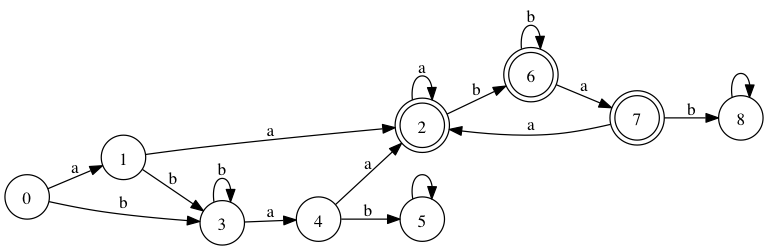
\includegraphics[width=\textwidth]{11-1.gv.png}
\end{figure}

\subsection{}
\begin{fancyquotes}
  Convert your finite automata from part $1a$ to a regular expression,
  by removing one vertex at a time. Show the resulting machine after
  each vertex is removed.
\end{fancyquotes}

\begin{figure}[hp]
  \centering
  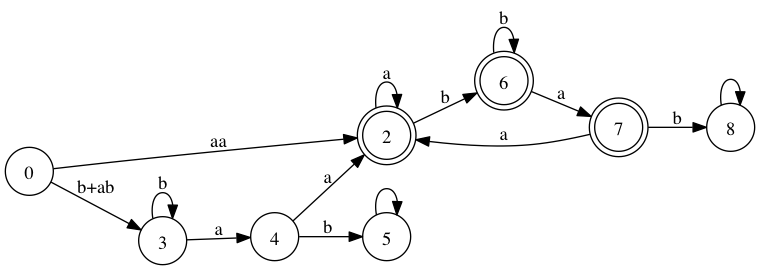
\includegraphics[width=.7\textwidth]{11-1.gv.2.png}
  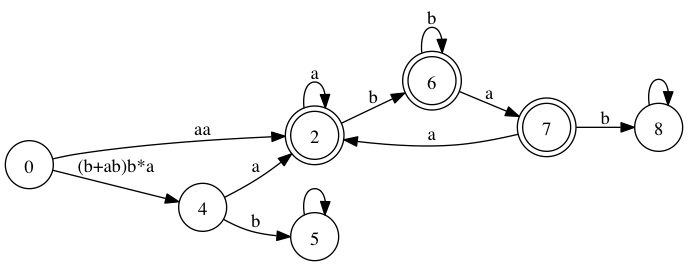
\includegraphics[width=.7\textwidth]{11-1.gv.3.png}
  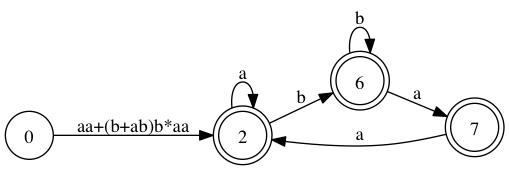
\includegraphics[width=.7\textwidth]{11-1.gv.4.png}
  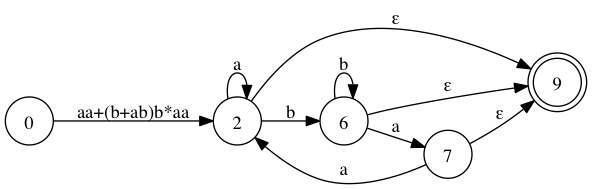
\includegraphics[width=.7\textwidth]{11-1.gv.5.png}
  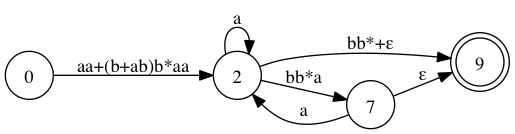
\includegraphics[width=.7\textwidth]{11-1.gv.6.png}
  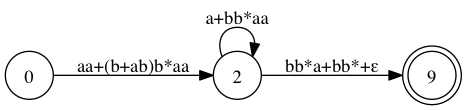
\includegraphics[width=.7\textwidth]{11-1.gv.7.png}
  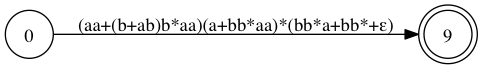
\includegraphics[width=.7\textwidth]{11-1.gv.8.png}
\end{figure}

\pagebreak

% -----------------------------------------------------------------------------
% PROBLEM 2
% -----------------------------------------------------------------------------
\section{}

\begin{fancyquotes}
  Show that the language $L$ is all strings over $\{0,1,2,3,4\}$ that
  represent base-5 numbers evenly divisible by $3$ is regular. So $0,
  3, 11, 14, 22 \in L$.
\end{fancyquotes}

This can be solved by DFA:

$$K = \{q_0, q_1, q_2\}$$
$$\Sigma = \{0,1,2,3,4\}$$
$$\Delta = (q_i\times j)\rightarrow q_{(5*i+j)\bmod 3}$$
$$s = q_0$$
$$F = \{q_0\}$$

So $L$ is regular.

\pagebreak

% -----------------------------------------------------------------------------
% PROBLEM 3
% -----------------------------------------------------------------------------
\section{}

\begin{fancyquotes}
  Show that the language $L$ is all strings over $\{a,b,+,*,(,)\}$
  represent valid regular expressions over the alphabet $\{a,b\}$ is
  Context-Free, but not regular.
\end{fancyquotes}

$$S \rightarrow SS$$
$$S \rightarrow (S)$$
$$S \rightarrow S+S$$
$$S \rightarrow S*$$
$$S \rightarrow a$$
$$S \rightarrow b$$
$$S \rightarrow \epsilon$$

So $L$ is Context-Free.
% Since $L$ needs to track the parentheses, it can't be regular.

Assume that $L$ is regular.

Let $n$ be the constant of the pumping lemma.

Given a string $w = (^{n}a)^{n}$, which $|w|>n$.

For every decomposition of $w=xyz$ such that $|xy|<n, |y|>0$.
Then:
$$x=(^{j}$$
$$y=(^{k}$$
$$z=(^{n-j-k}a)^{n}$$

Let $i=2$, then $w_2=xy^{i}z=xy^2z=(^{n+k}a)^{n}$ which $w_2\not\in
L$.

So $L$ is not regular.

\pagebreak

% -----------------------------------------------------------------------------
% PROBLEM 4
% -----------------------------------------------------------------------------
\section{}

\begin{fancyquotes}
  Show that both of the following decision problems are in $P$:
\end{fancyquotes}

\subsection{}
\begin{fancyquotes}
  DNF-Satisfiability: Given a Boolean expression in disjunctive normal
  form (the disjunction of clauses, each of which is a conjunction of
  literals) is satisfiable.

  DNF Example: The formula $f=(x_1\wedge
  x_2)\vee(x_3\wedge\overline{x_4}\wedge x_5)\vee(\overline{x_2}\wedge
  x_3)$ is in disjunctive normal form.
\end{fancyquotes}

Since all the clauses are conjuncted by OR operation,
and in any clause its variables appears only once,
we can simply pick an arbitrary clause and set all variables inside to
be true, to make the total DNF to be satisfiable.

The time cost is $O(n)$, which $n$ is the length of the DNF\@.

So the problem is in $P$.

\subsection{}
\begin{fancyquotes}
  CNF-Tautology: Given a boolean expression in Conjunctive Normal
  Form, is it a tautology (that is, is it true under any truth
  assignment of its variables)?
\end{fancyquotes}

Since all the clauses are conjuncted by AND operation,
all the clauses have to be TRUE to make the whole CNF to be TRUE\@.
If the CNF is tautology, it means all the clauses are tautology.
Inside the clauses are the variables conjuncted by OR operation,
so if they are tautology, then for every clause there exists some
variable $x$, both $x,\overline{x}$ are in the clause.

The time cost to check it is $O(n)$, which $n$ is the length of the
CNF\@.

So the problem is in $P$.

\pagebreak

% -----------------------------------------------------------------------------
% PROBLEM 5
% -----------------------------------------------------------------------------
\section{}

\begin{fancyquotes}
   Question 7.1.1 from the text

   In 3-COLORING we are given an undirected graph, and we are asked
   whether its nodes can be colored with three colors such that no two
   adjacent nodes have the same color.
\end{fancyquotes}

\subsection{}
\begin{fancyquotes}
  Show that 3-COLORING is in NP\@.
\end{fancyquotes}

For a given solution, just do DFS on the solution to check all the
edges whether two adjacent nodes have the same color.

\subsection{}
\begin{fancyquotes}
  Describe a polynomial-time reduction from 3-COLORING to
  SATISFIABILITY\@.
\end{fancyquotes}

We are trying to use SATISFIABILITY solver to solve 3-COLORING
problem.

Assume we have three colors $a,b,c$.

For every node $x_i$ in the coloring problem graph,
generate three variables as node+color:
$$(x_i, a)$$
$$(x_i, b)$$
$$(x_i, c)$$

Every node $x_i$ has only one color:
$$((x_i,a) \vee (x_i,b) \vee (x_i,c))$$
$$(\overline{(x_i,a)} \vee \overline{(x_i,b)})$$
$$(\overline{(x_i,a)} \vee \overline{(x_i,c)})$$
$$(\overline{(x_i,b)} \vee \overline{(x_i,c)})$$

For every edge $(x_i,x_j)$ in the graph,
ajacent nodes $x_i, x_j$ have different colors:
$$(\overline{(x_i,a)} \vee \overline{(x_j,a)})$$
$$(\overline{(x_i,b)} \vee \overline{(x_j,b)})$$
$$(\overline{(x_i,c)} \vee \overline{(x_j,c)})$$

We can generate these clauses in polynomial-time.
Then we can use SATISFIABILITY solver to solve the problem.

\pagebreak

\end{document}